
\newpage

\section{Github + Travis CI - \ \  \"{} the pdflatex way \"{}}
\subsection{Was wird benötigt ?}
{\color{green}Kostenlose} Variante (nur public Repo's):
\begin{itemize}
  \item Ein Github - Account
  \item Ein Travis-CI (.org) Account
  \item Das Travis Command-line Tool
\end{itemize}
\vspace{0.5cm}
{\color{red}Kostenpflichtige} / Studenten Variante \\(Auch private Repo's / und sofortige build's):
\begin{itemize}
  \item Ein kostenpflichtiger Github - Account ( \$7/ Monat)
  \item Ein kostenpflichtiger Travis-CI (.com) Account ( \$69/ Monat)
  \item Alternativ ein Student Developer Pack von Github \\ siehe: https://education.github.com/pack
  \item Das Travis Command-line Tool
\end{itemize}


%
%   Seite 4
%
%   Github
%
\newpage
\subsection{Einrichtung}
\subsection{Github}
Als erstes benötigen wir einen Github Account inkl. Repo.
\begin{center}
  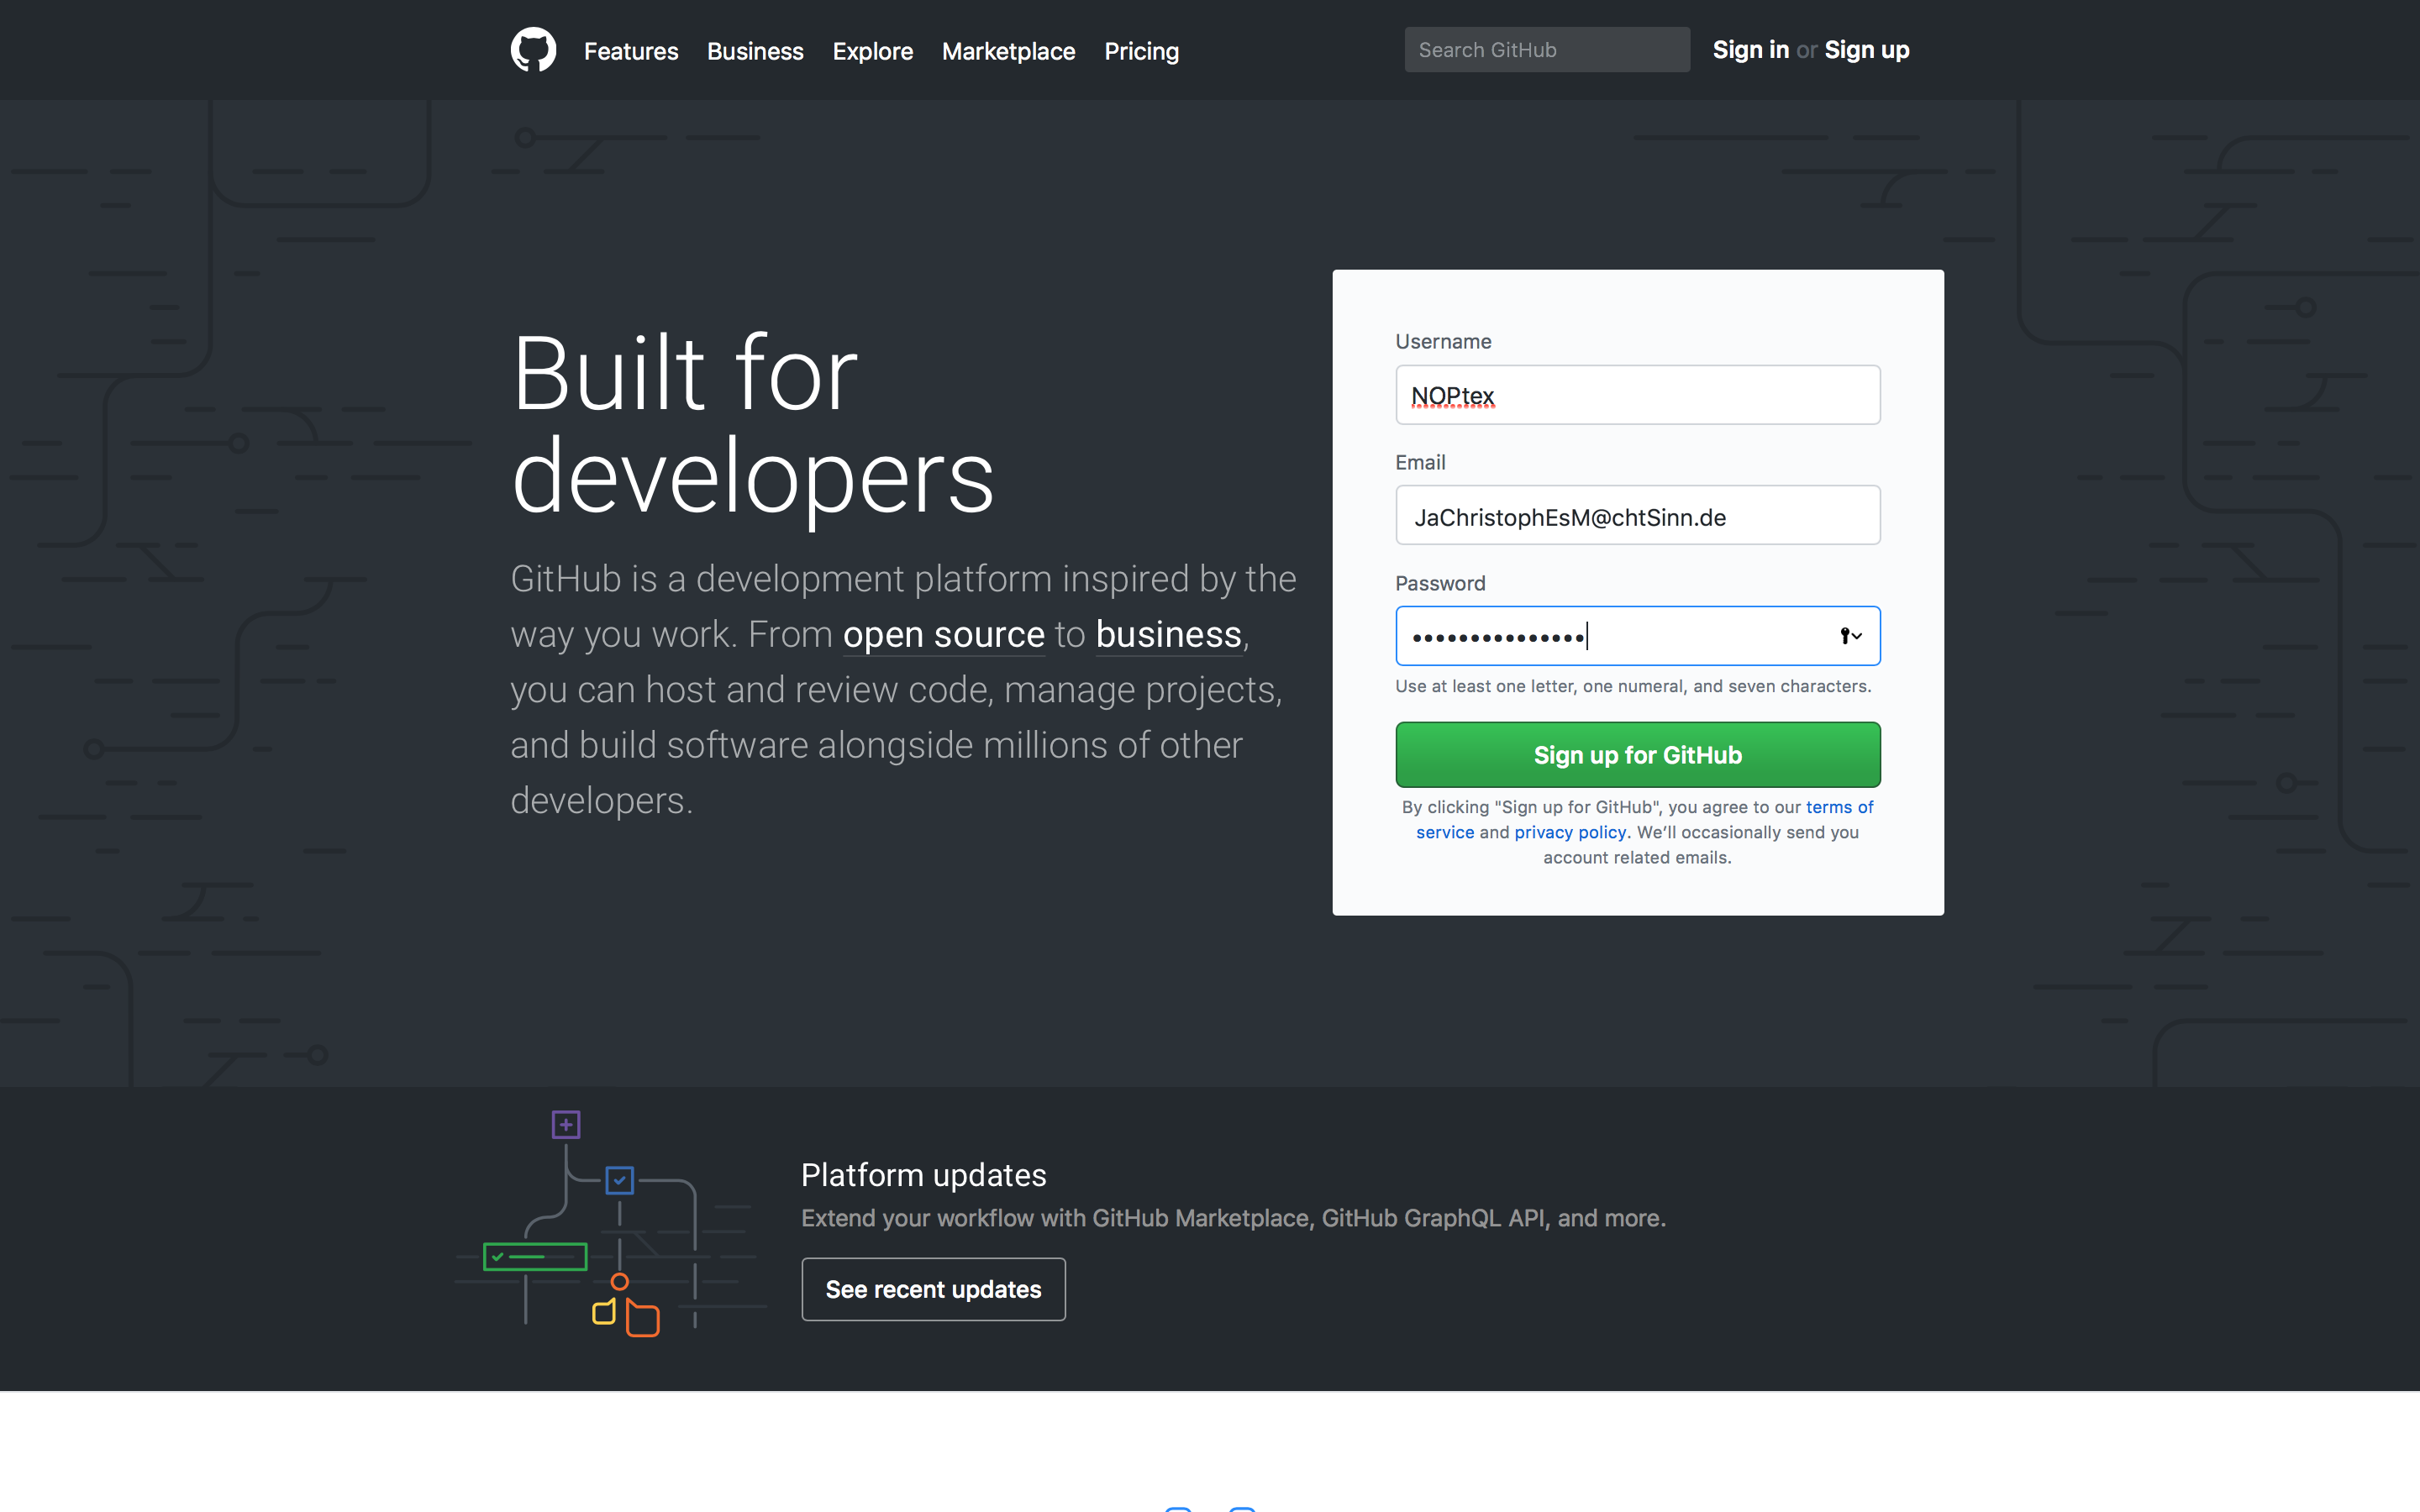
\includegraphics[trim = 300px 10px 300px 0px, clip,height=11cm]{./bilder/1Github.png}
\end{center}

% "l, b, r, t"
% \begin{figure}
% 	\centering
% \end{figure}\includegraphics[trim = 20px 10px 20px 30px, clip, width=\textwidth]{Beispiel.jpg}
% 	\caption{Hier steht der Beschriftungstext.}
% 	\label{fig:Beispiel}
% \end{figure}



\newpage
(Im Verlauf dieses Vortrages verwende ich:\\

https://github.com/NOPtex/NOP)\\


Dort befindet sich ein funktionierender Prototyp. \\
(Welcher aber noch ein paar zusätzlich Dateien beinhaltet.) \\

Prinzipiell reicht eine \TeX -Datei und die .travis.yml.

\begin{center}
  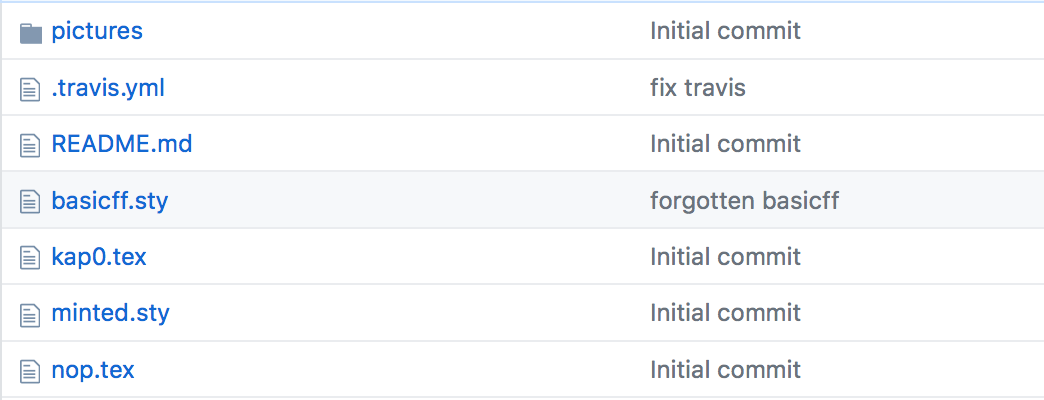
\includegraphics[width=0.8\textwidth]{./bilder/2Boilerplate.png}
\end{center}

%
%
% \vspace{0.5cm}
%
% \begin{center}
%   \includegraphics[width=1.0\textwidth]{./bilder/plainRepo.png}
% \end{center}

%
%   Seite 5
%
%   Github
% \cleardoublepage

\newpage % ============================================= Newpage ===================


\begin{figure}[ht]
  \subsection{Travis CI}
  \subsubsection{In Travis CI einloggen und mit Github verbinden}
\adjustbox{valign=t}{\begin{minipage}[t]{0.50\textwidth}
\begin{framed}
  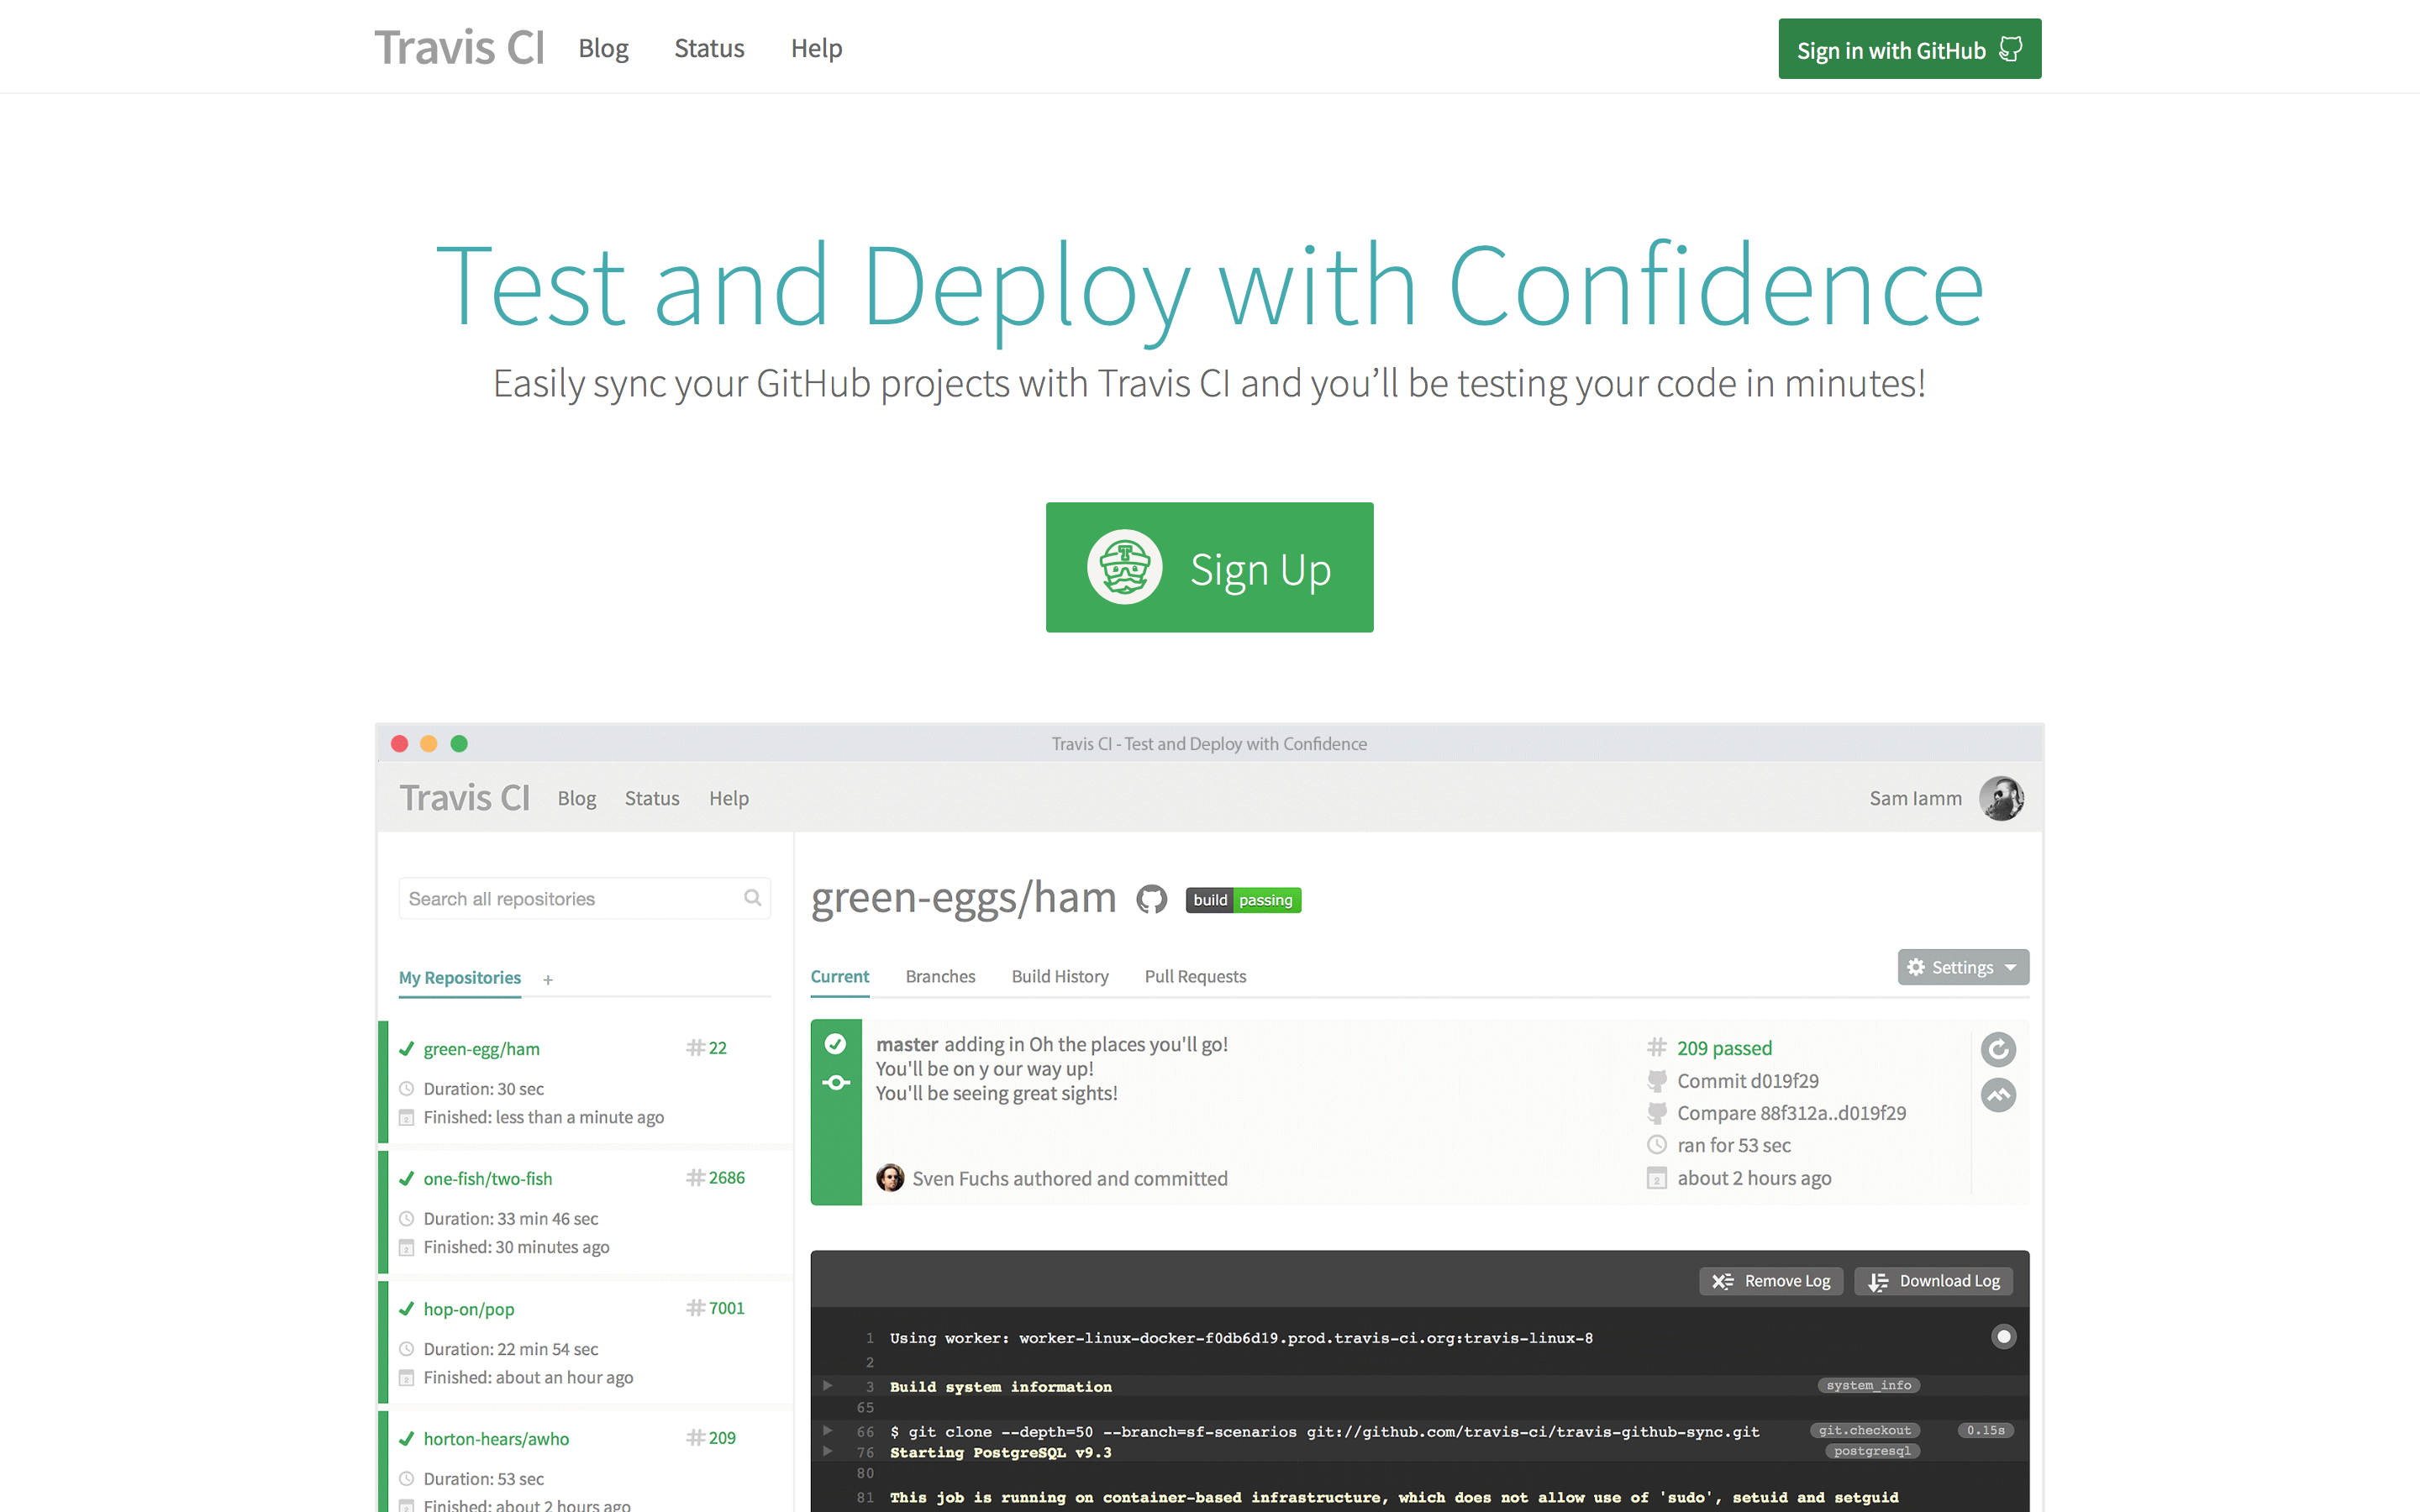
\includegraphics[width=1.0\textwidth]{./bilder/3travisSignUP.png}
\end{framed}

\end{minipage}}
% \hfill
\adjustbox{valign=t}{\begin{minipage}[t]{0.45\textwidth}
\vspace{0pt}
\huge
Da Travis nur mit Github \\funktioniert ist die Einrichtung recht \"{}trivial\"{}.
% \caption{Kapazität}
\end{minipage}}
% \end{figure}
% \vspace{0.5cm} % ----------------------------------- vspace
% \begin{figure}[ht]
\adjustbox{valign=t}{\begin{minipage}[t]{0.50\textwidth}
% \vspace{0.5cm}
\begin{framed}
  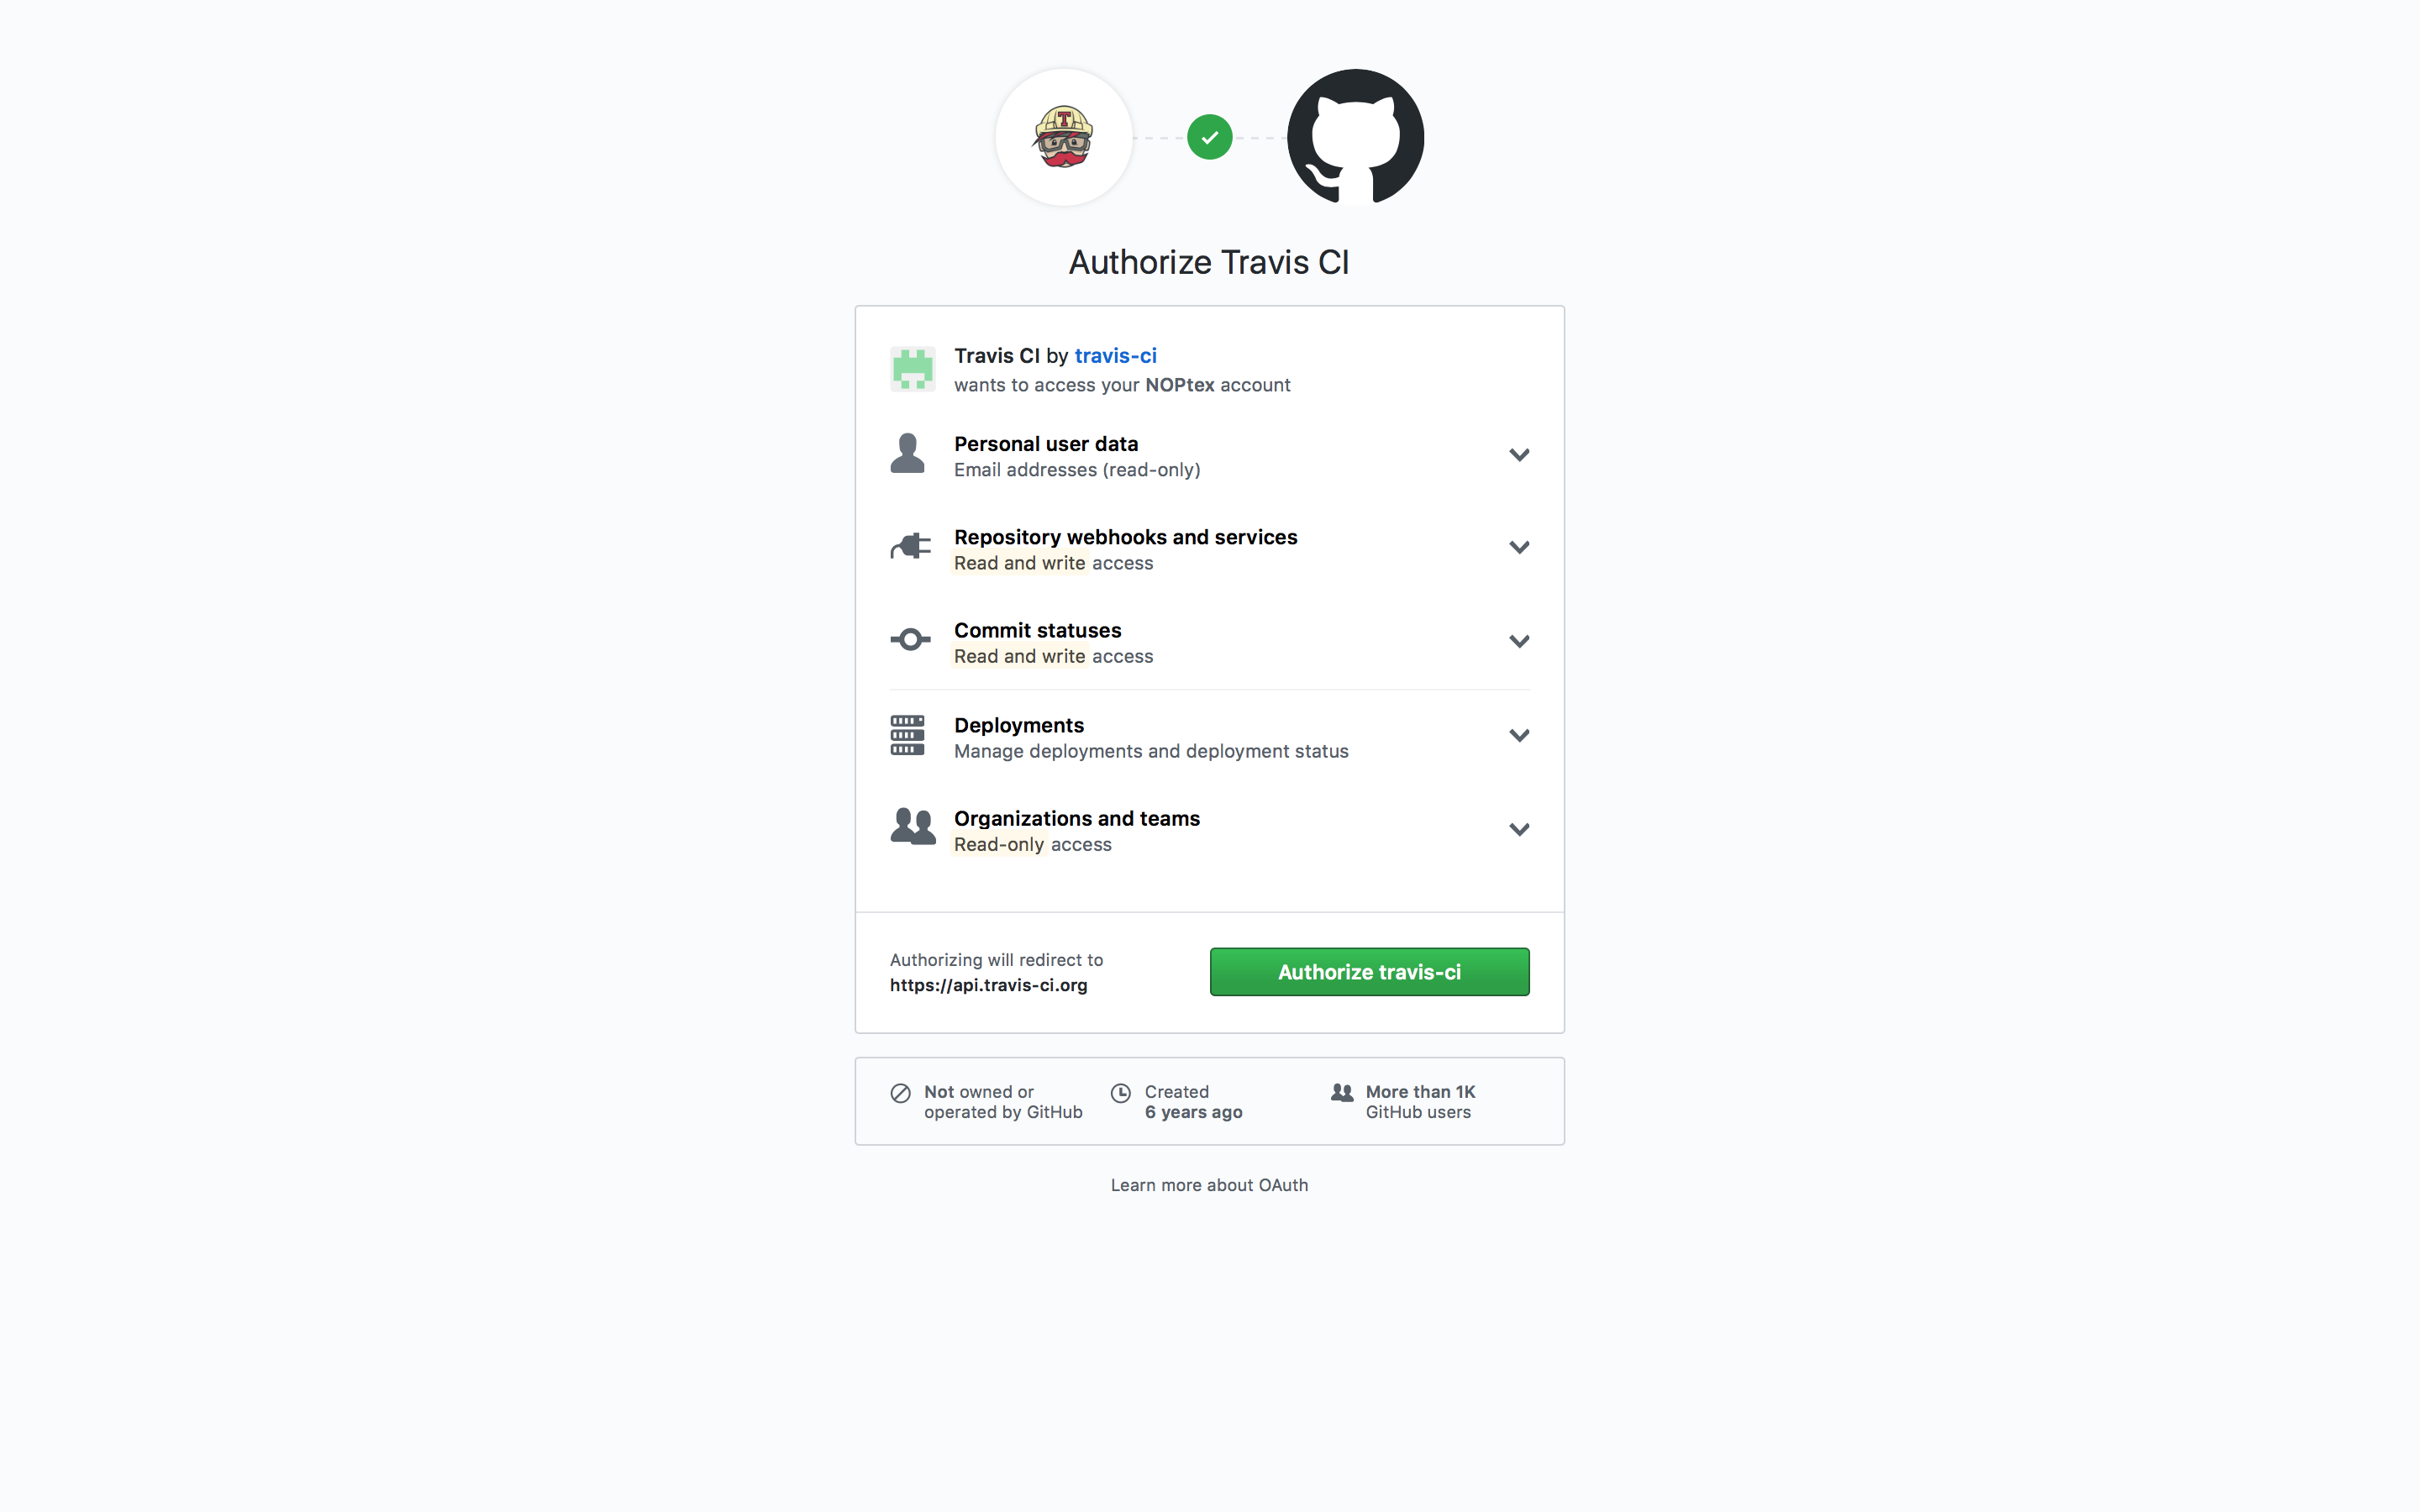
\includegraphics[width=1.0\textwidth]{./bilder/4TRAVISauthGITHUB.png}
\end{framed}

\end{minipage}}
\hfill
\adjustbox{valign=t}{\begin{minipage}[t]{0.45\textwidth}
\vspace{0pt}
\huge
Travis benötigt einige \\Berechtigungen welche man in diesem Schritt erteilt.
% \caption{Kapazität}
\end{minipage}}
\end{figure}

\clearpage % GleitObjekte anzeigen






\newpage % ============================================= Newpage ===================


\begin{figure}[ht]
  \subsubsection{Github - Repo aktivieren}
\adjustbox{valign=t}{\begin{minipage}[t]{0.50\textwidth}
\begin{framed}
  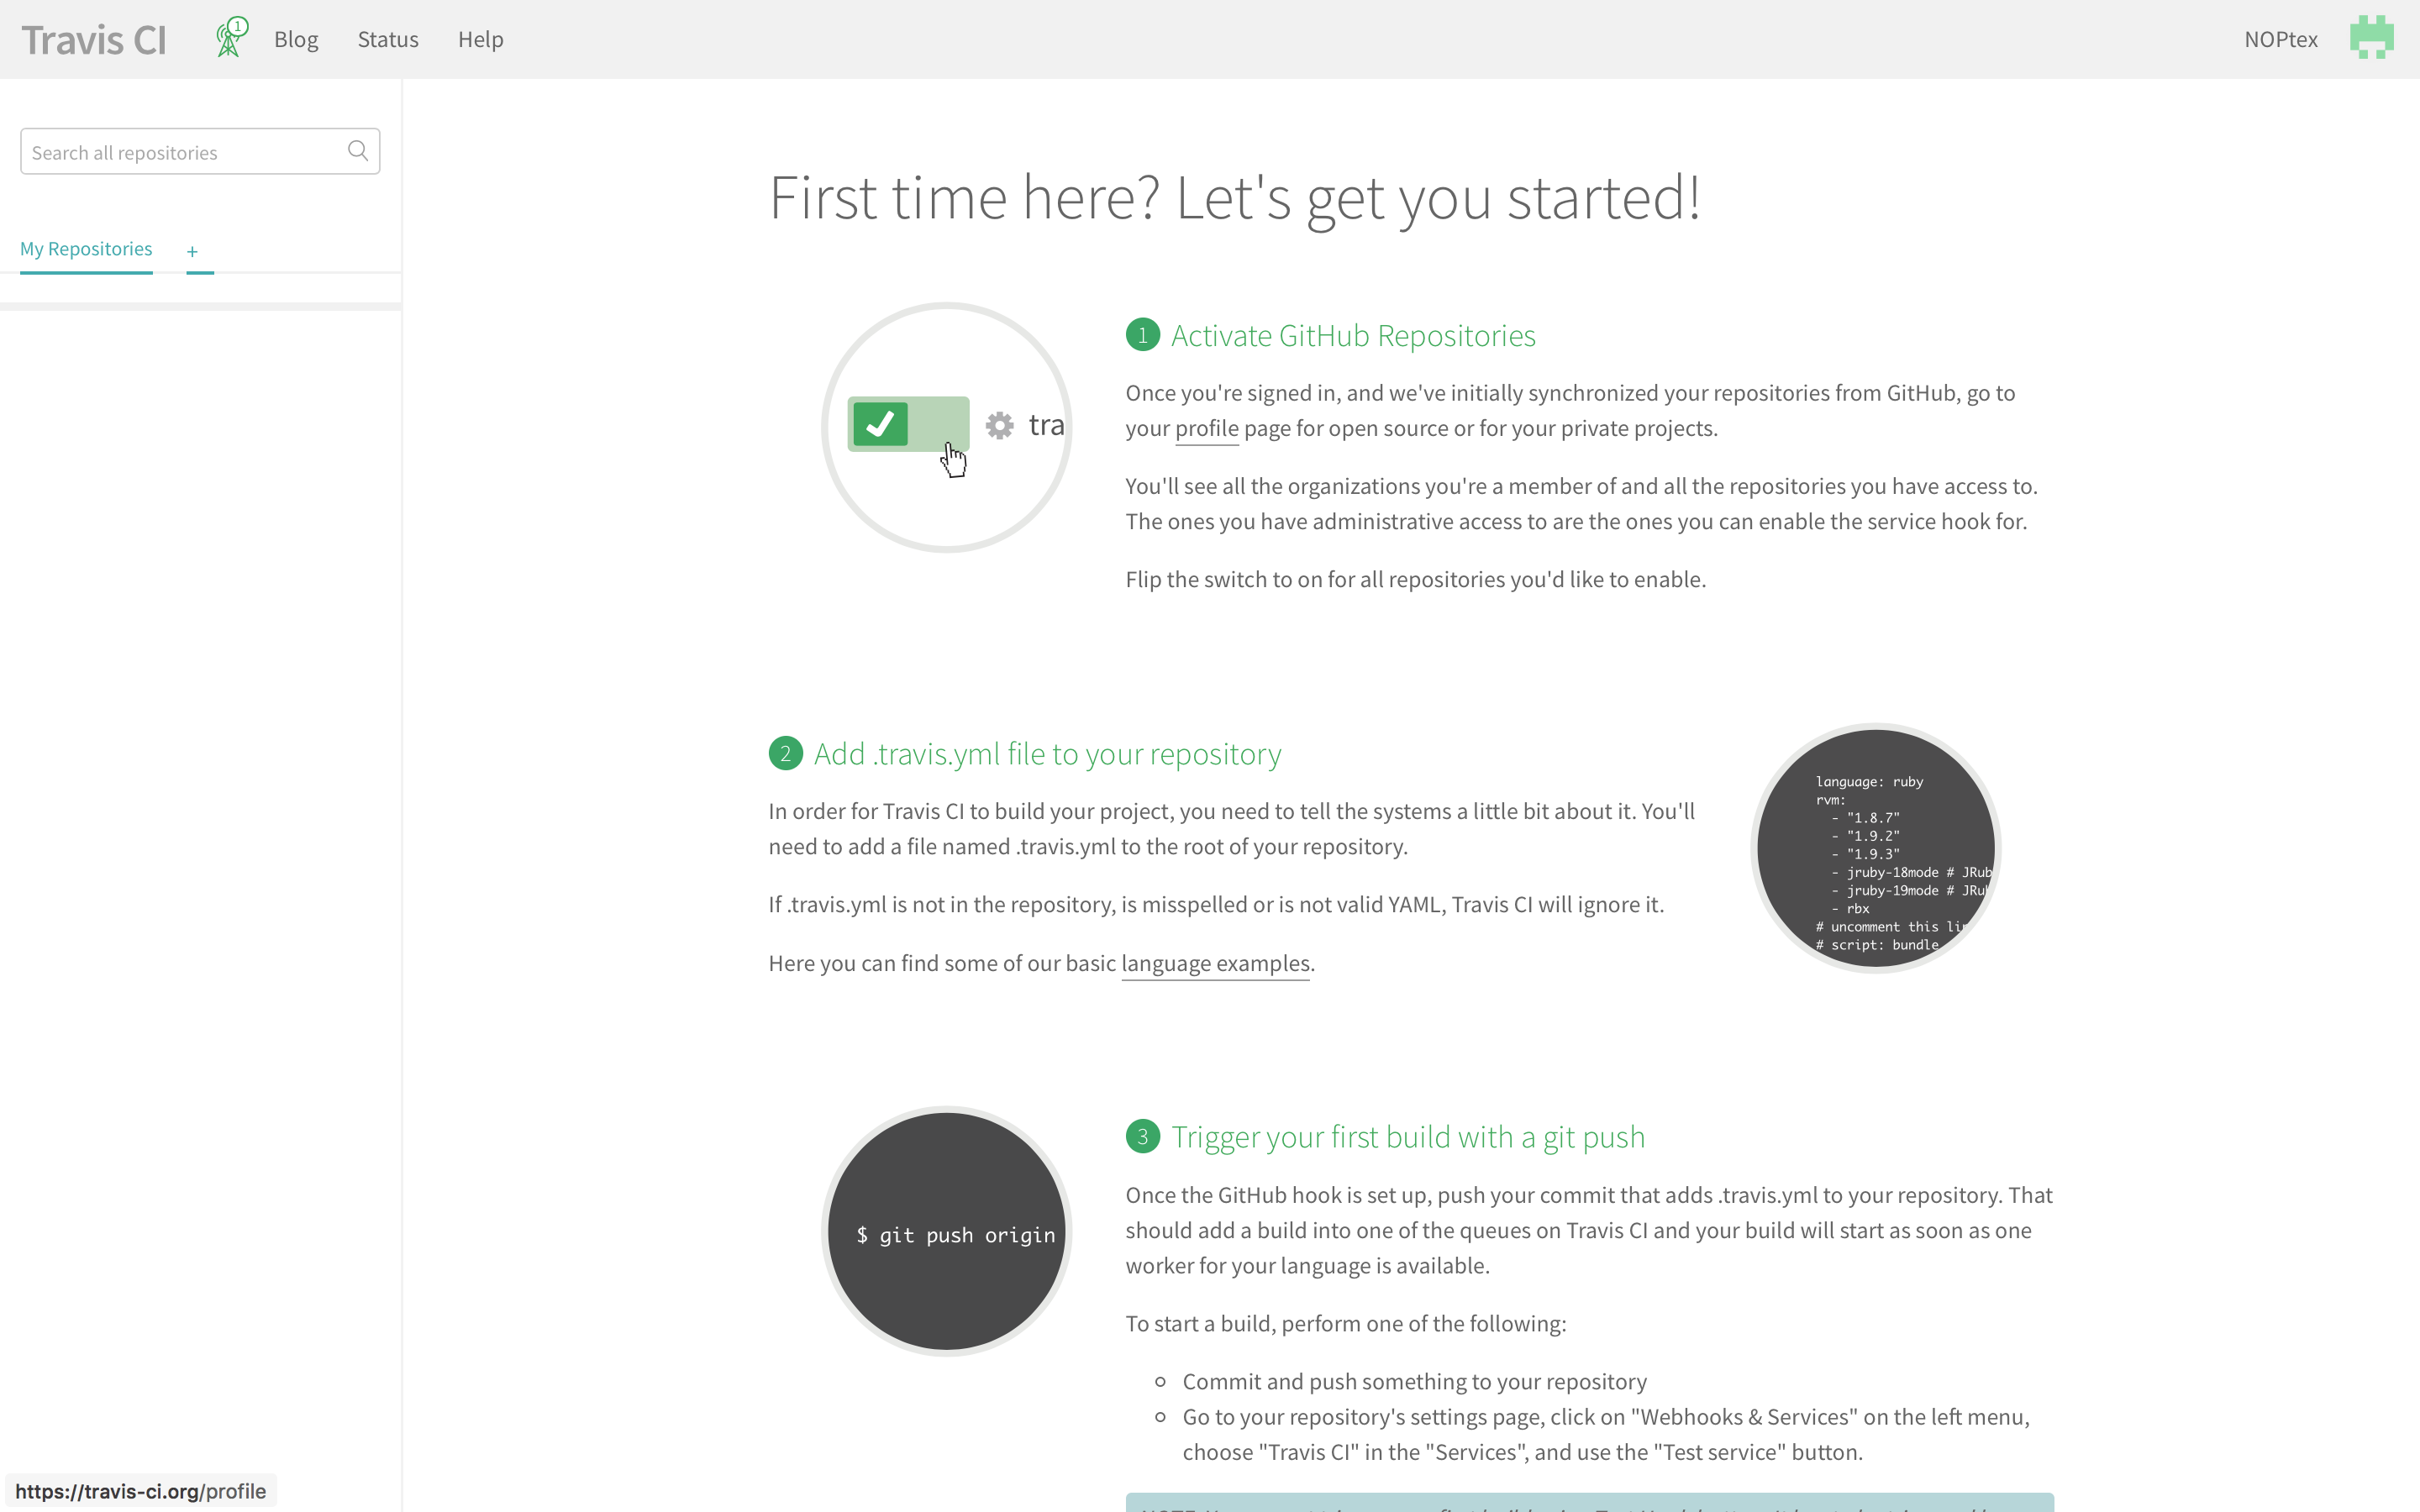
\includegraphics[width=1.0\textwidth]{./bilder/5TRAVISfirstSignIn.png}
\end{framed}

\end{minipage}}
% \hfill
\adjustbox{valign=t}{\begin{minipage}[t]{0.45\textwidth}
\vspace{0pt}
\huge
Da Travis nur mit Github funktioniert ist die Einrichtung recht einfach.
% \caption{Kapazität}
\end{minipage}}
% \end{figure}
% \vspace{0.5cm} % ----------------------------------- vspace
% \begin{figure}[ht]
\adjustbox{valign=t}{\begin{minipage}[t]{0.50\textwidth}
% \vspace{0.5cm}
\begin{framed}
  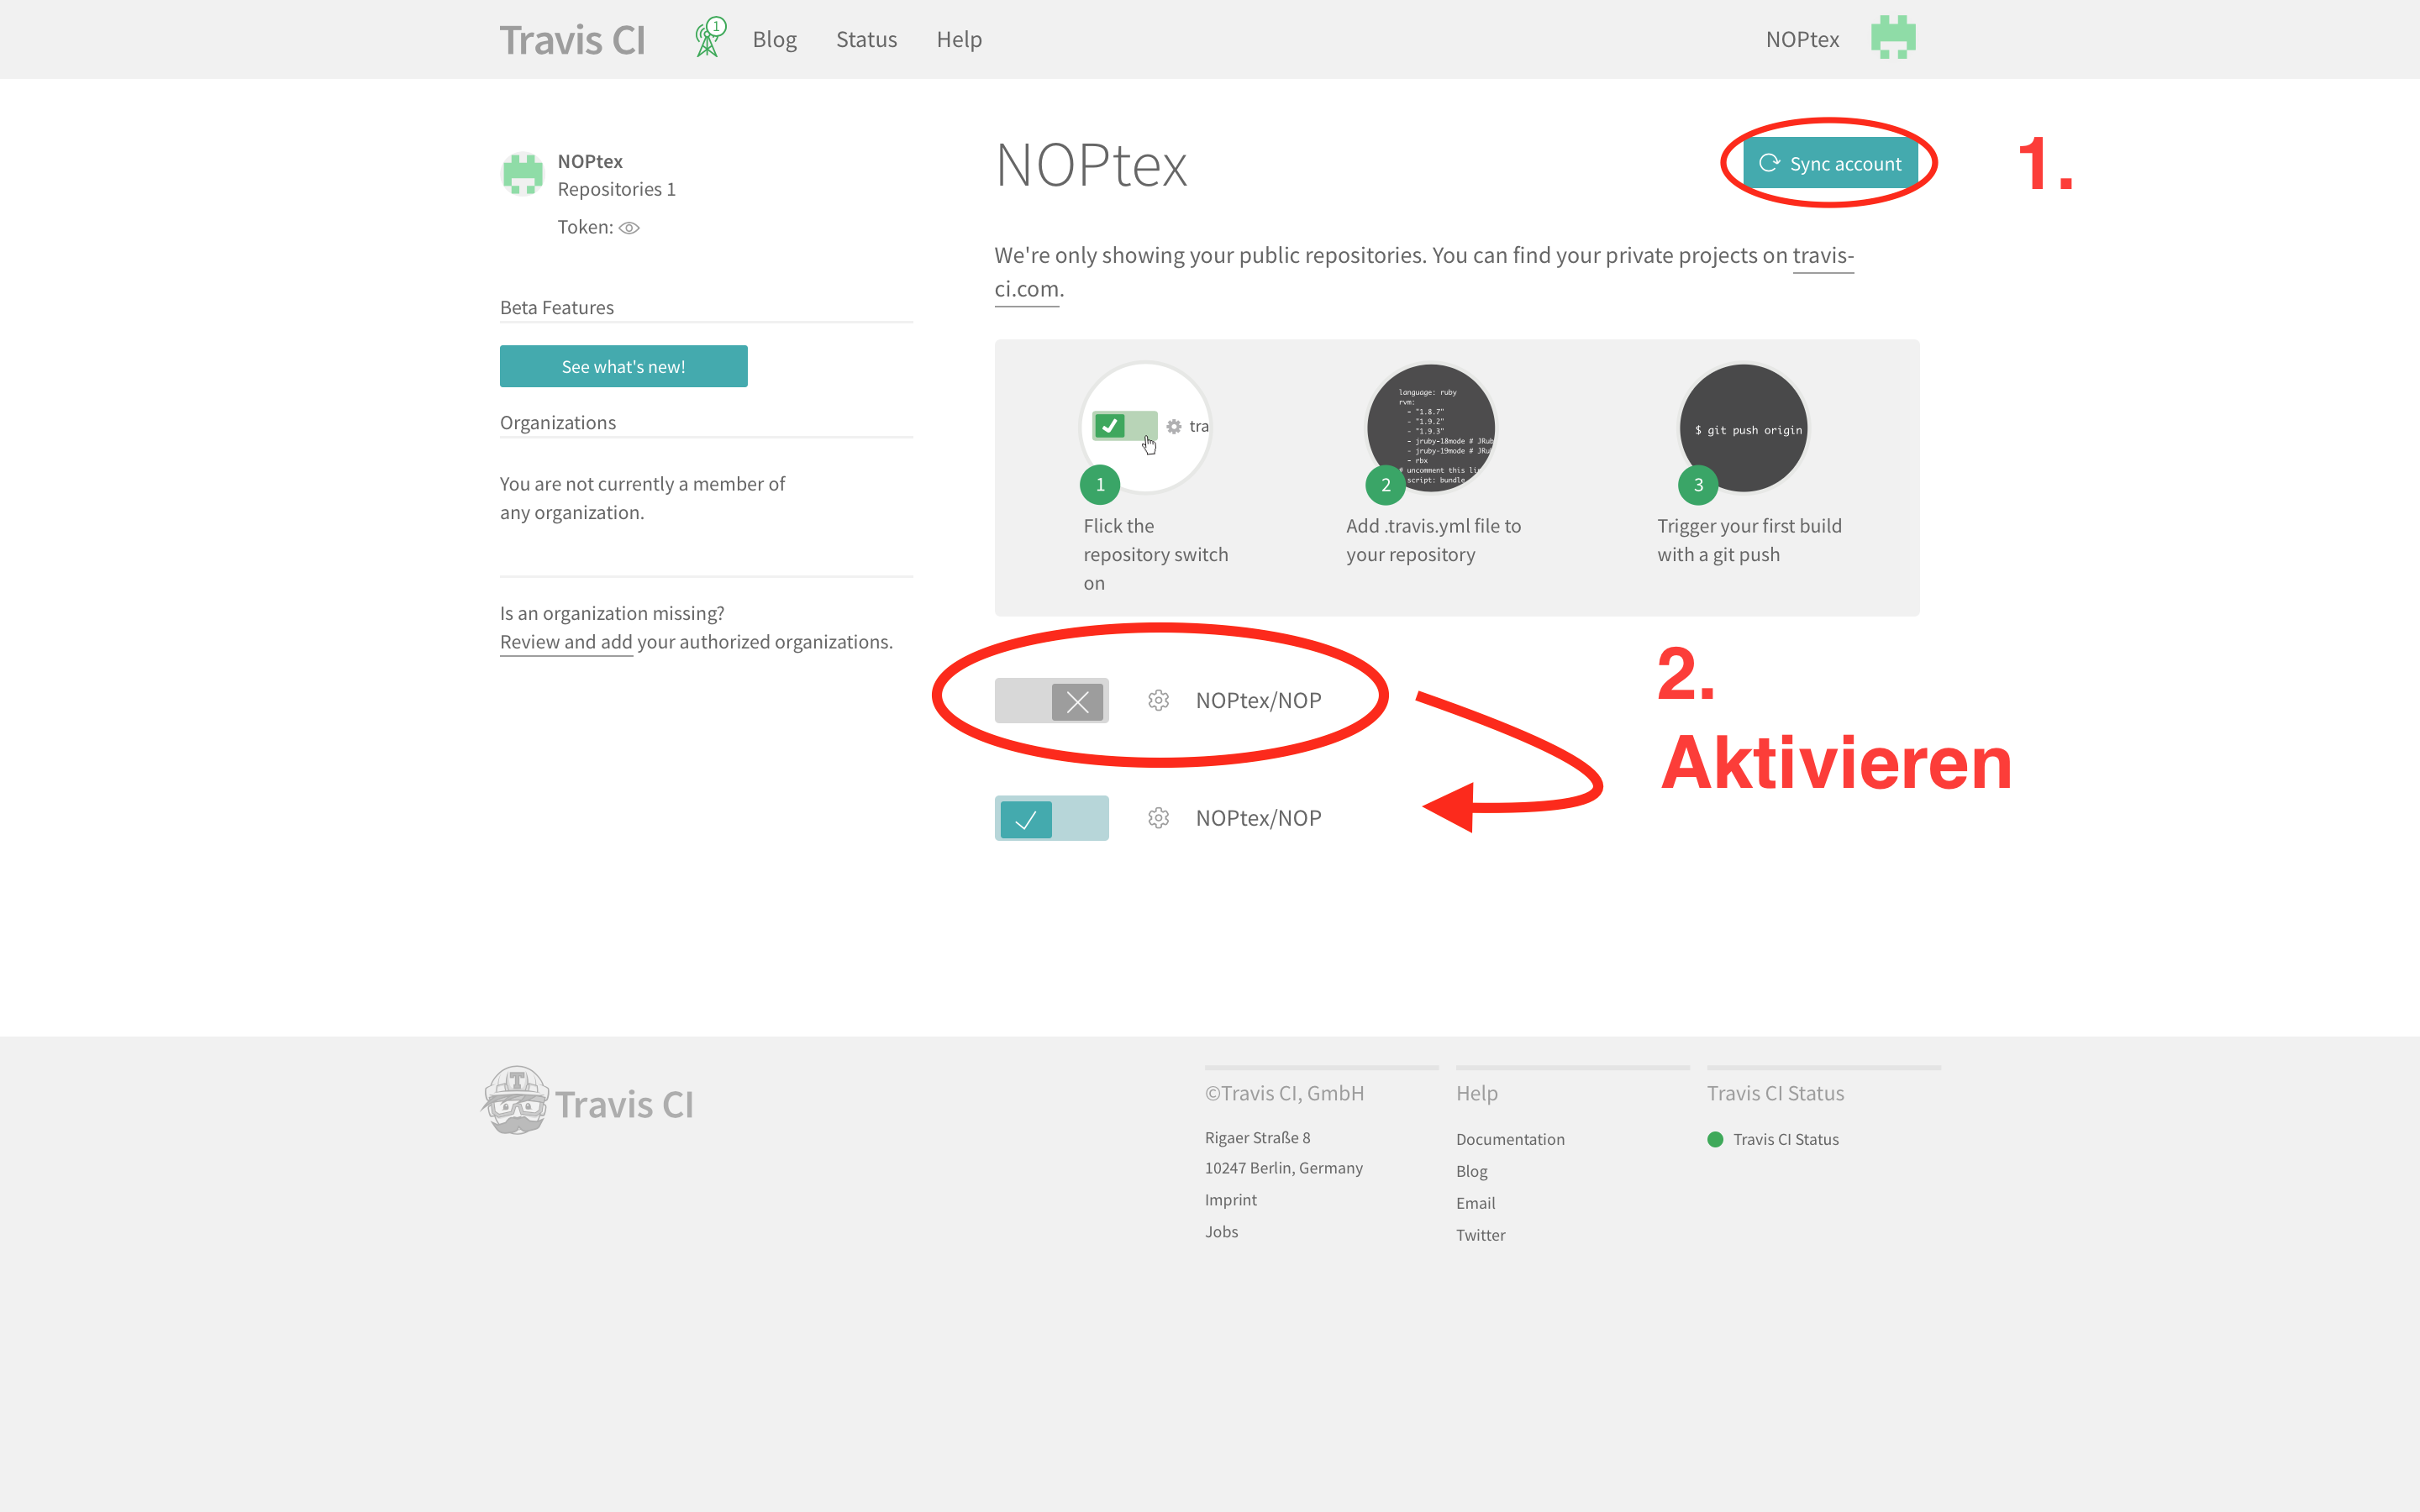
\includegraphics[width=1.0\textwidth]{./bilder/6TRAVISActivateREPO.png}
\end{framed}

\end{minipage}}
\hfill
\adjustbox{valign=t}{\begin{minipage}[t]{0.45\textwidth}
\vspace{0pt}
\huge
Travis benötigt einige Berechtigungen welche man im nächsten Schritt erteilt.
% \caption{Kapazität}
\end{minipage}}
\end{figure}

\clearpage % GleitObjekte anzeigen


\newpage % ============================================= Newpage ===================


\begin{figure}[ht]
  \subsubsection{Build-Einstellungen setzen}
\adjustbox{valign=t}{\begin{minipage}[t]{0.50\textwidth}
\begin{framed}
  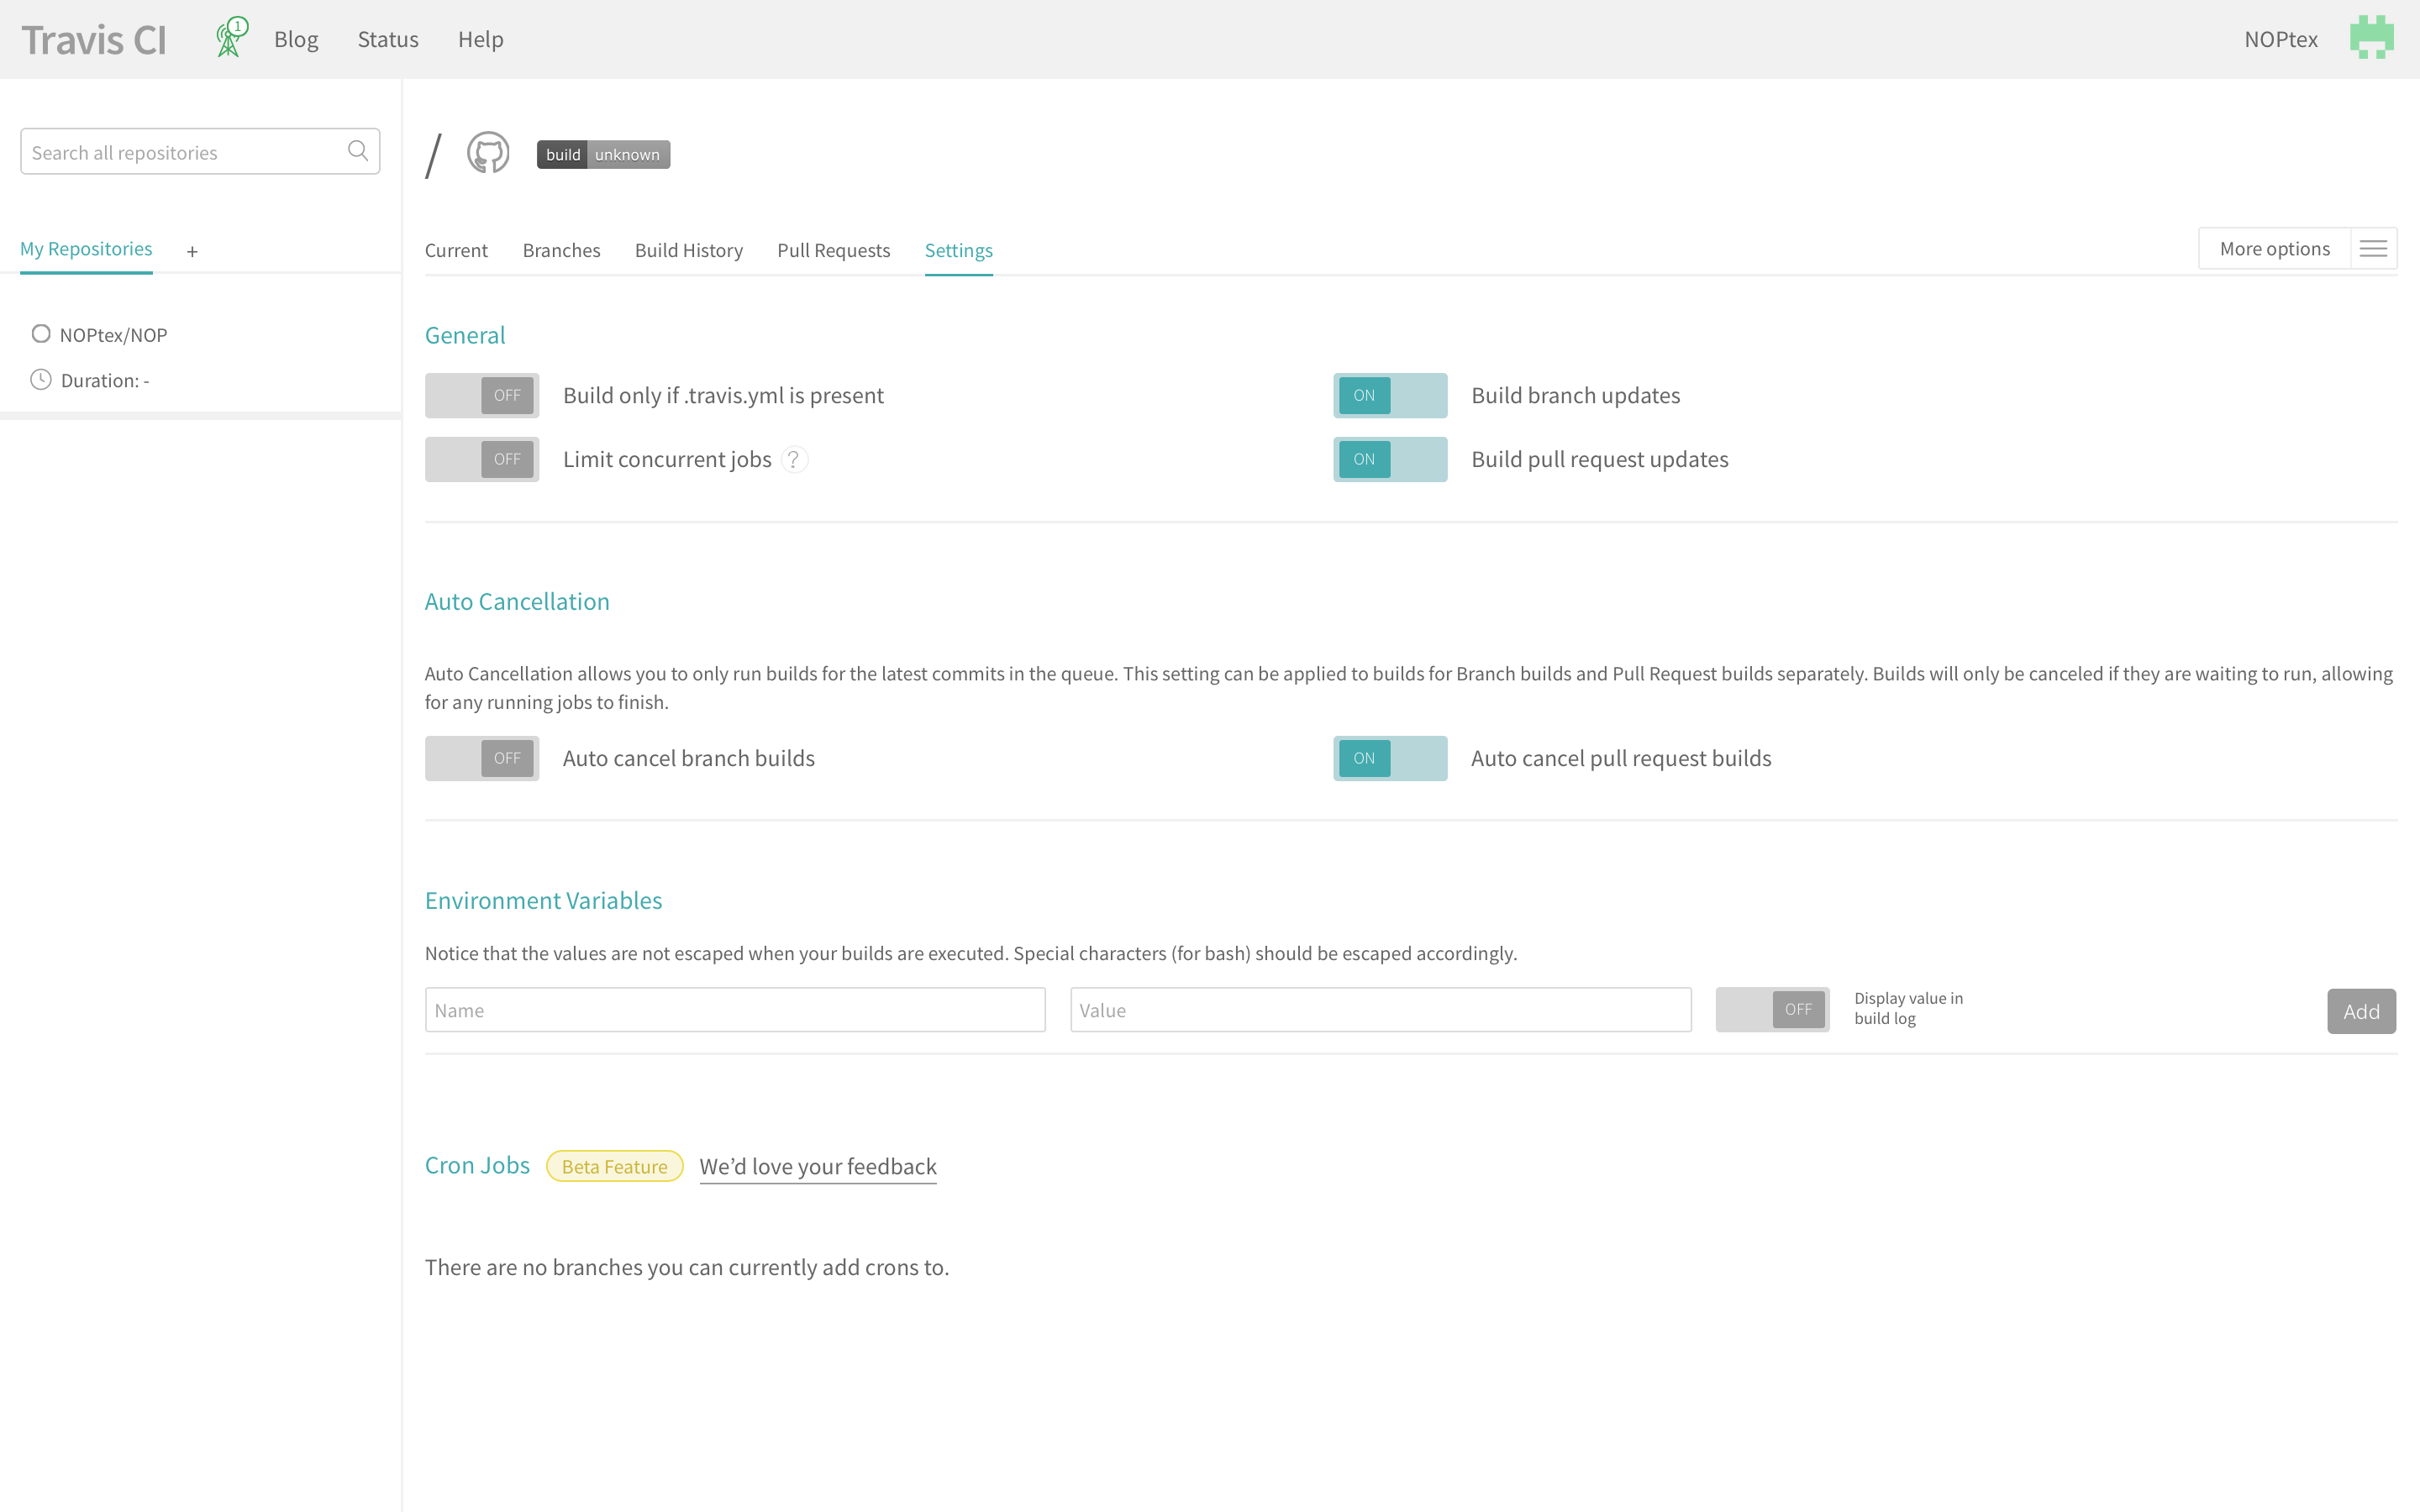
\includegraphics[width=1.0\textwidth]{./bilder/7TRAVISOptionsbase.png}
\end{framed}

\end{minipage}}
% \hfill
\adjustbox{valign=t}{\begin{minipage}[t]{0.45\textwidth}
\vspace{0pt}

\includegraphics[width=1.0\textwidth]{./bilder/7_1REPOsettings.png}
\huge
Über das Zahnrad kommt man zu den Einstellungen.
% \caption{Kapazität}
\end{minipage}}
% \end{figure}
% \vspace{0.5cm} % ----------------------------------- vspace
% \begin{figure}[ht]
\adjustbox{valign=t}{\begin{minipage}[t]{0.50\textwidth}
% \vspace{0.5cm}
\begin{framed}
  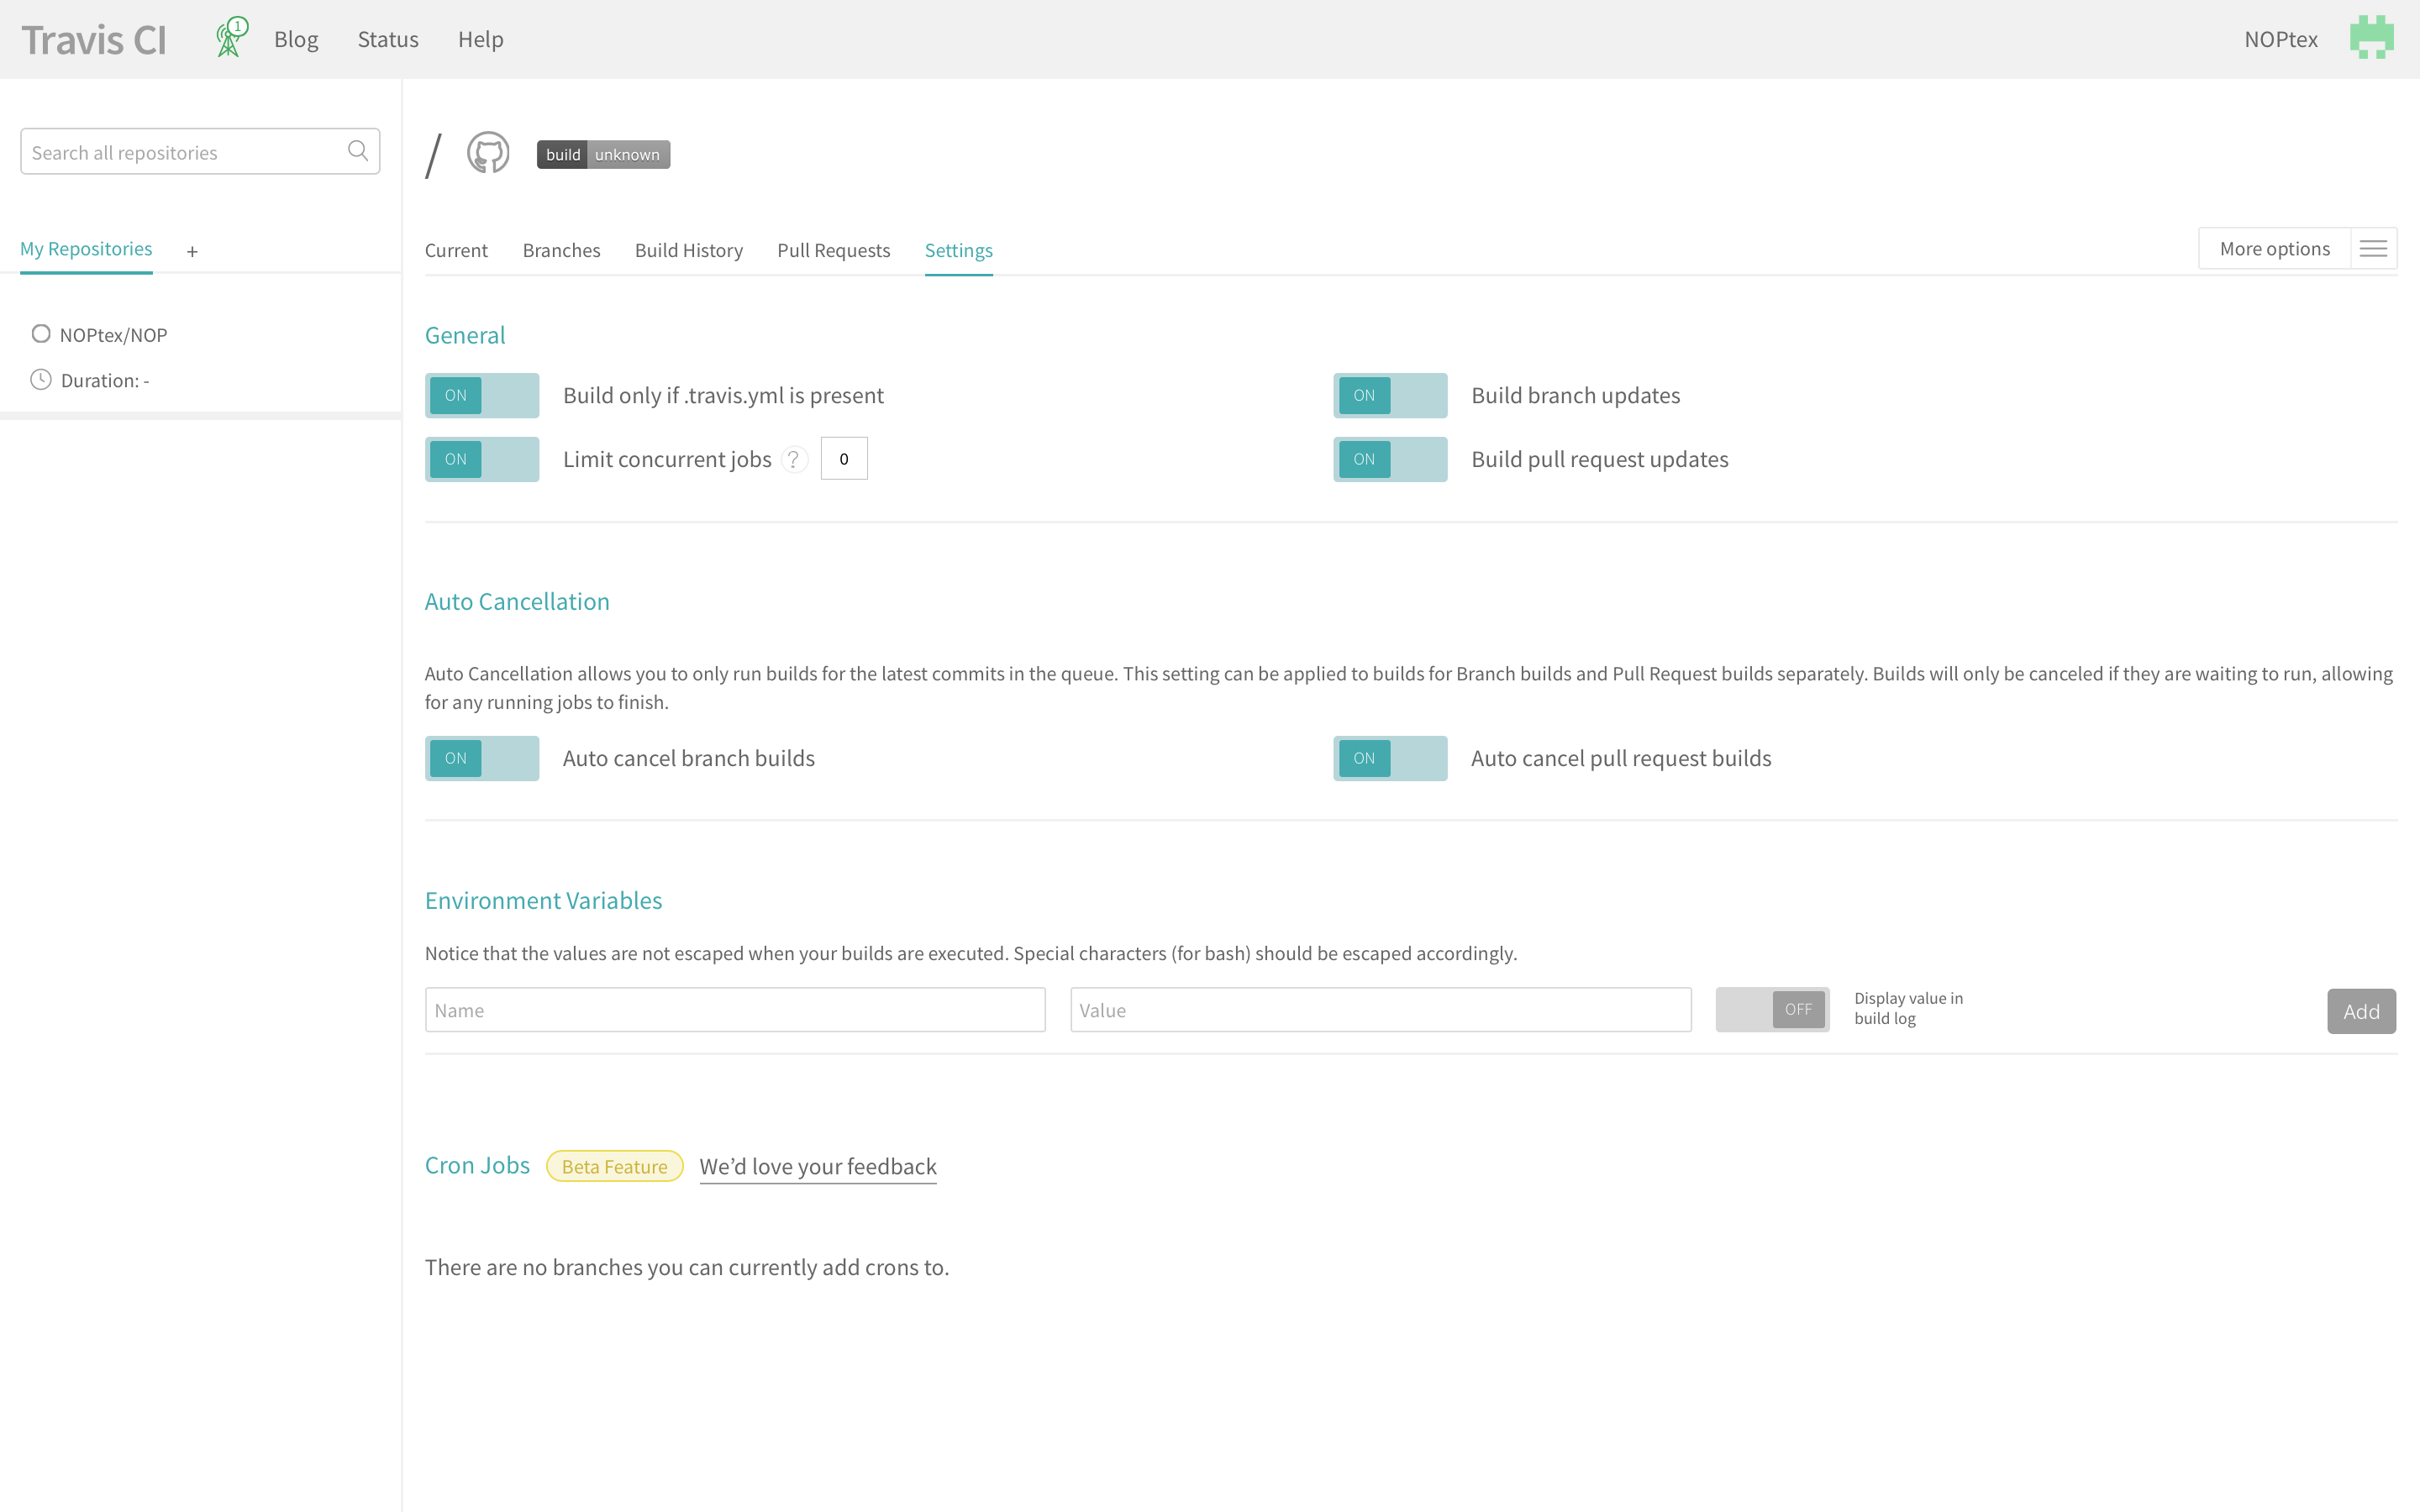
\includegraphics[width=1.0\textwidth]{./bilder/8TRAVISOptionsSET.png}
\end{framed}

\end{minipage}}
\hfill
\adjustbox{valign=t}{\begin{minipage}[t]{0.45\textwidth}
\vspace{0pt}
\huge
Ich setze alle Häkchen weil:
\begin{itemize}
  \item nur releases Gebaut werden sollen \\ (Testen kann man lokal) \\ Alle anderen Build sollen abgebrochen werden.
  \item Nur wenn .travis.yml vorhanden ist Build starten. \\(Einfaches deaktivieren über Git)
\end{itemize}
% \caption{Kapazität}
\end{minipage}}
\end{figure}

\clearpage % GleitObjekte anzeigen


%
% \newpage % ============================================= Newpage ===================
%
%
% \begin{figure}[ht]
%   \subsubsection{Build-Einstellungen setzen}
% \adjustbox{valign=t}{\begin{minipage}[t]{0.50\textwidth}
% \begin{framed}
%   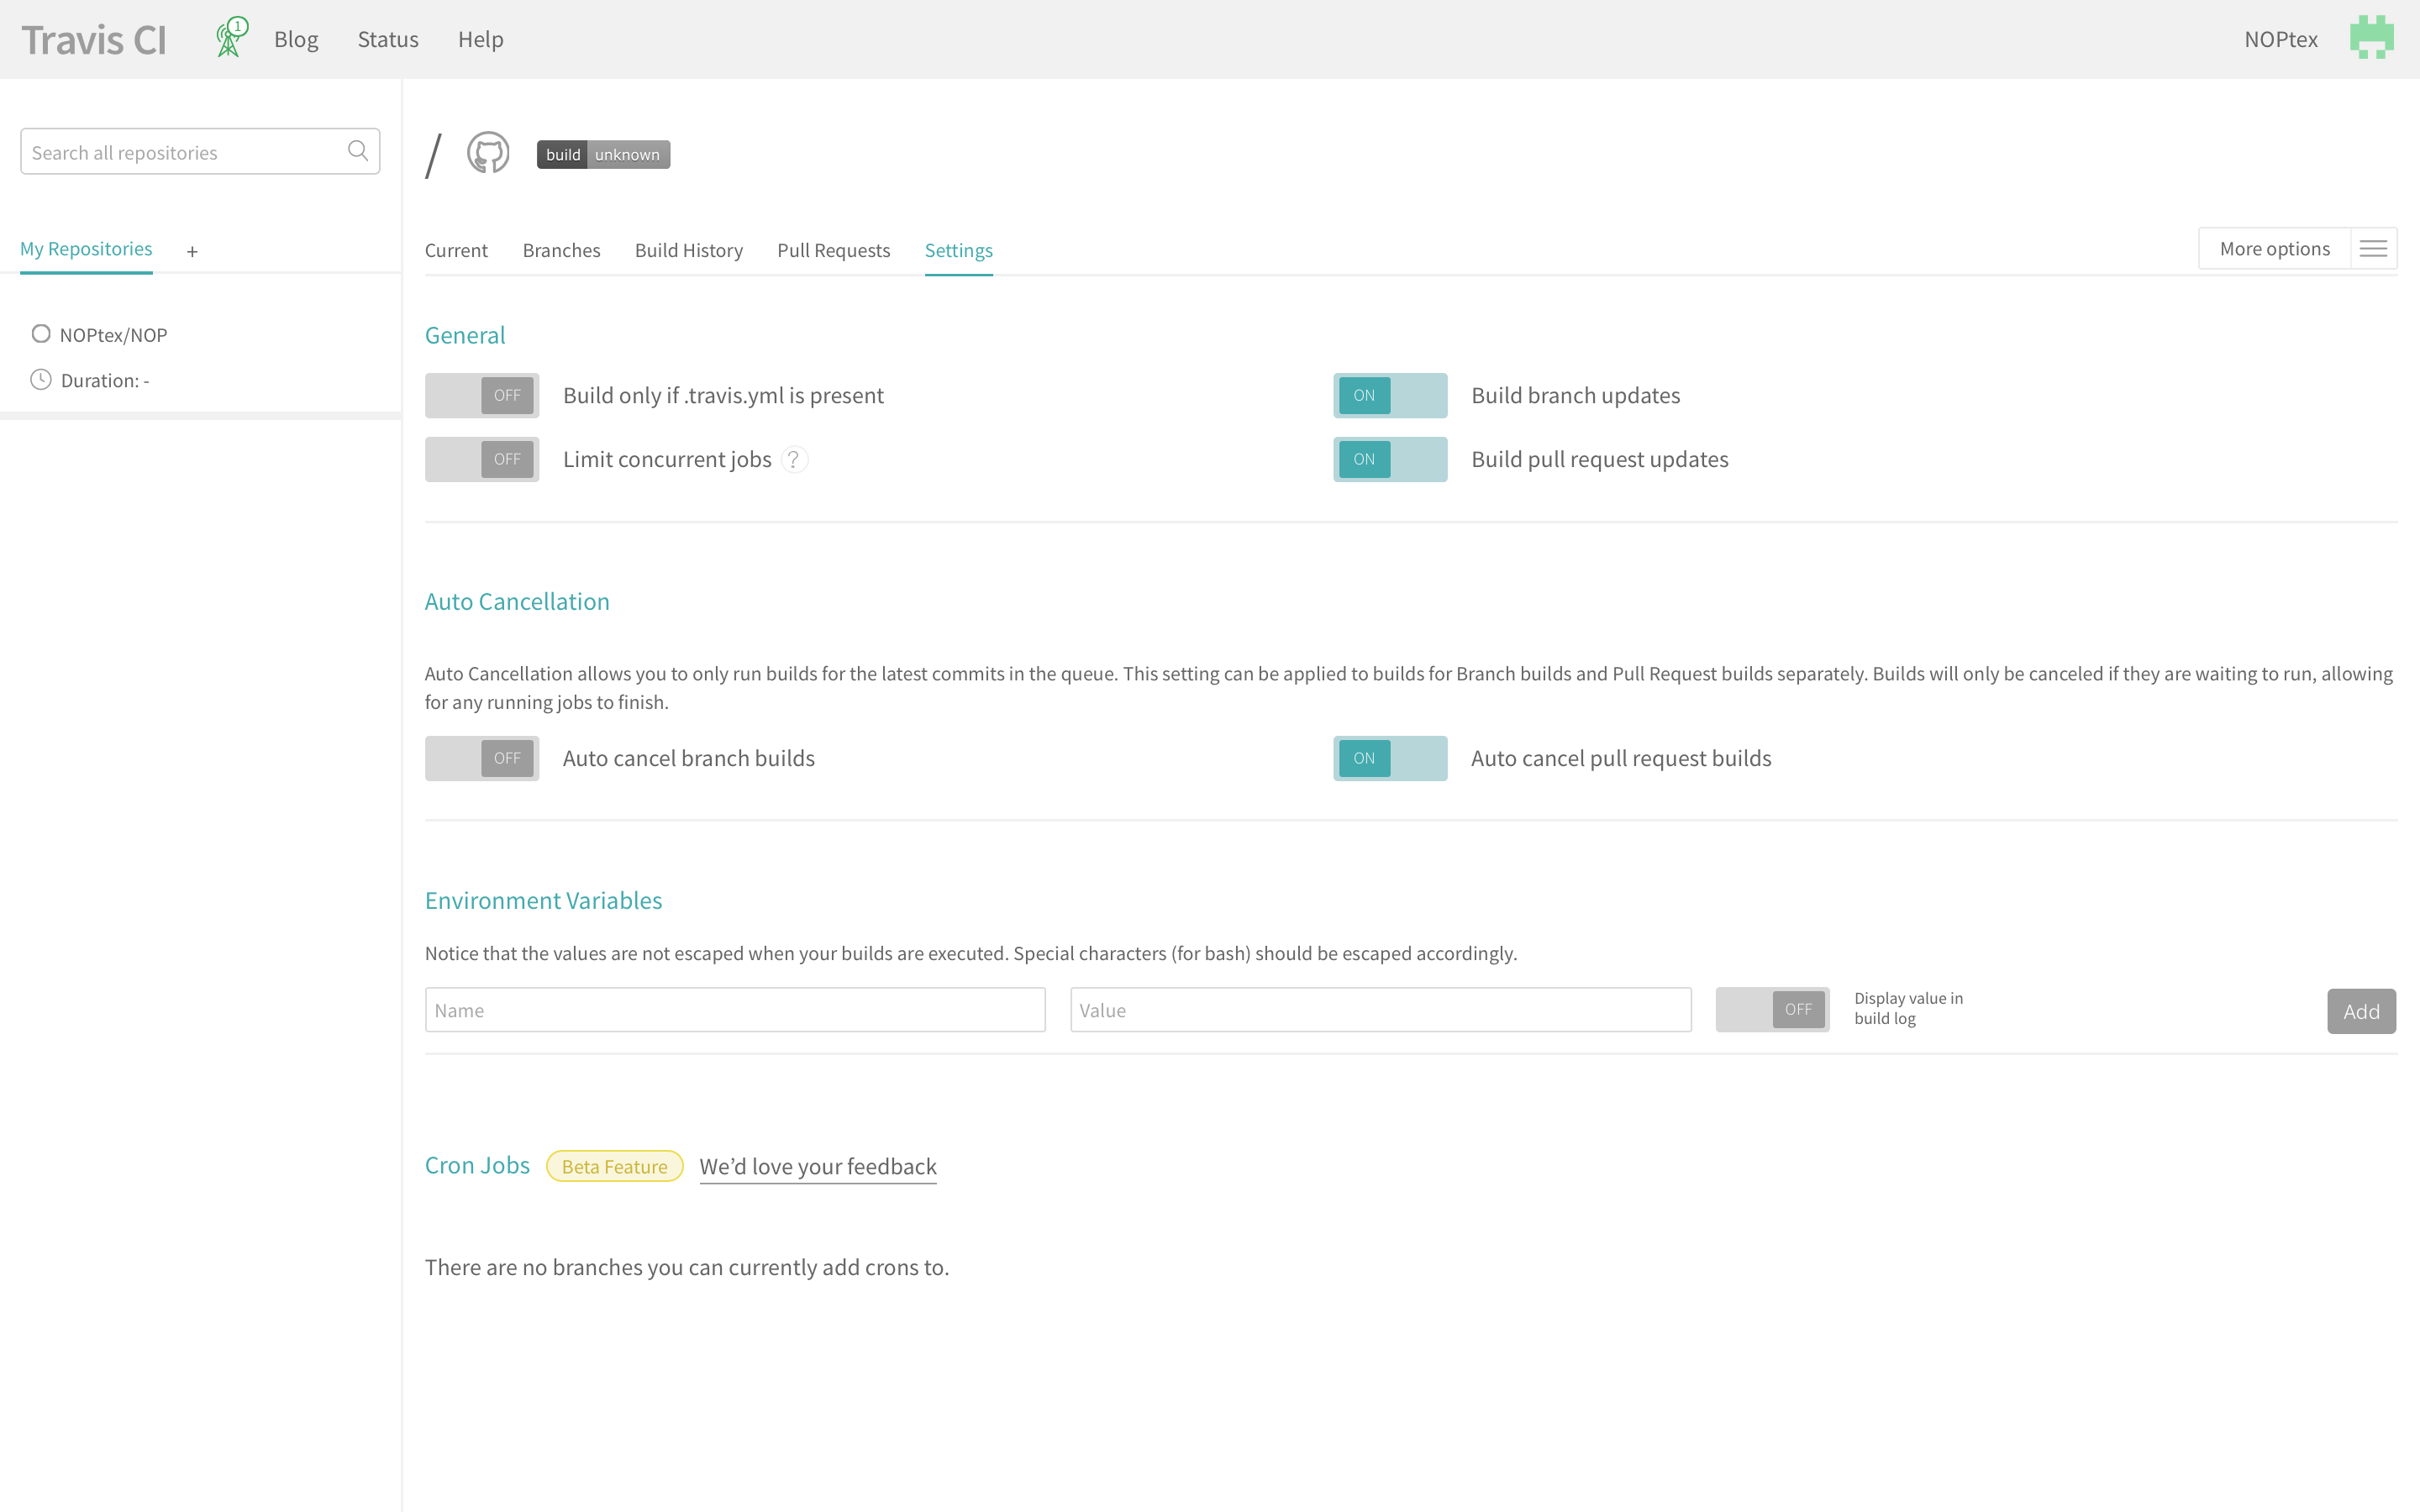
\includegraphics[width=1.0\textwidth]{./bilder/7TRAVISOptionsbase.png}
% \end{framed}
%
% \end{minipage}}
% % \hfill
% \adjustbox{valign=t}{\begin{minipage}[t]{0.45\textwidth}
% \vspace{0pt}
% 
\includegraphics[width=1.0\textwidth]{./bilder/7_1REPOsettings.png}
% \huge
% Über das Zahnrad kommt man zu den Einstellungen.
% % \caption{Kapazität}
% \end{minipage}}
% % \end{figure}
% % \vspace{0.5cm} % ----------------------------------- vspace
% % \begin{figure}[ht]
% \adjustbox{valign=t}{\begin{minipage}[t]{0.50\textwidth}
% % \vspace{0.5cm}
% \begin{framed}
%   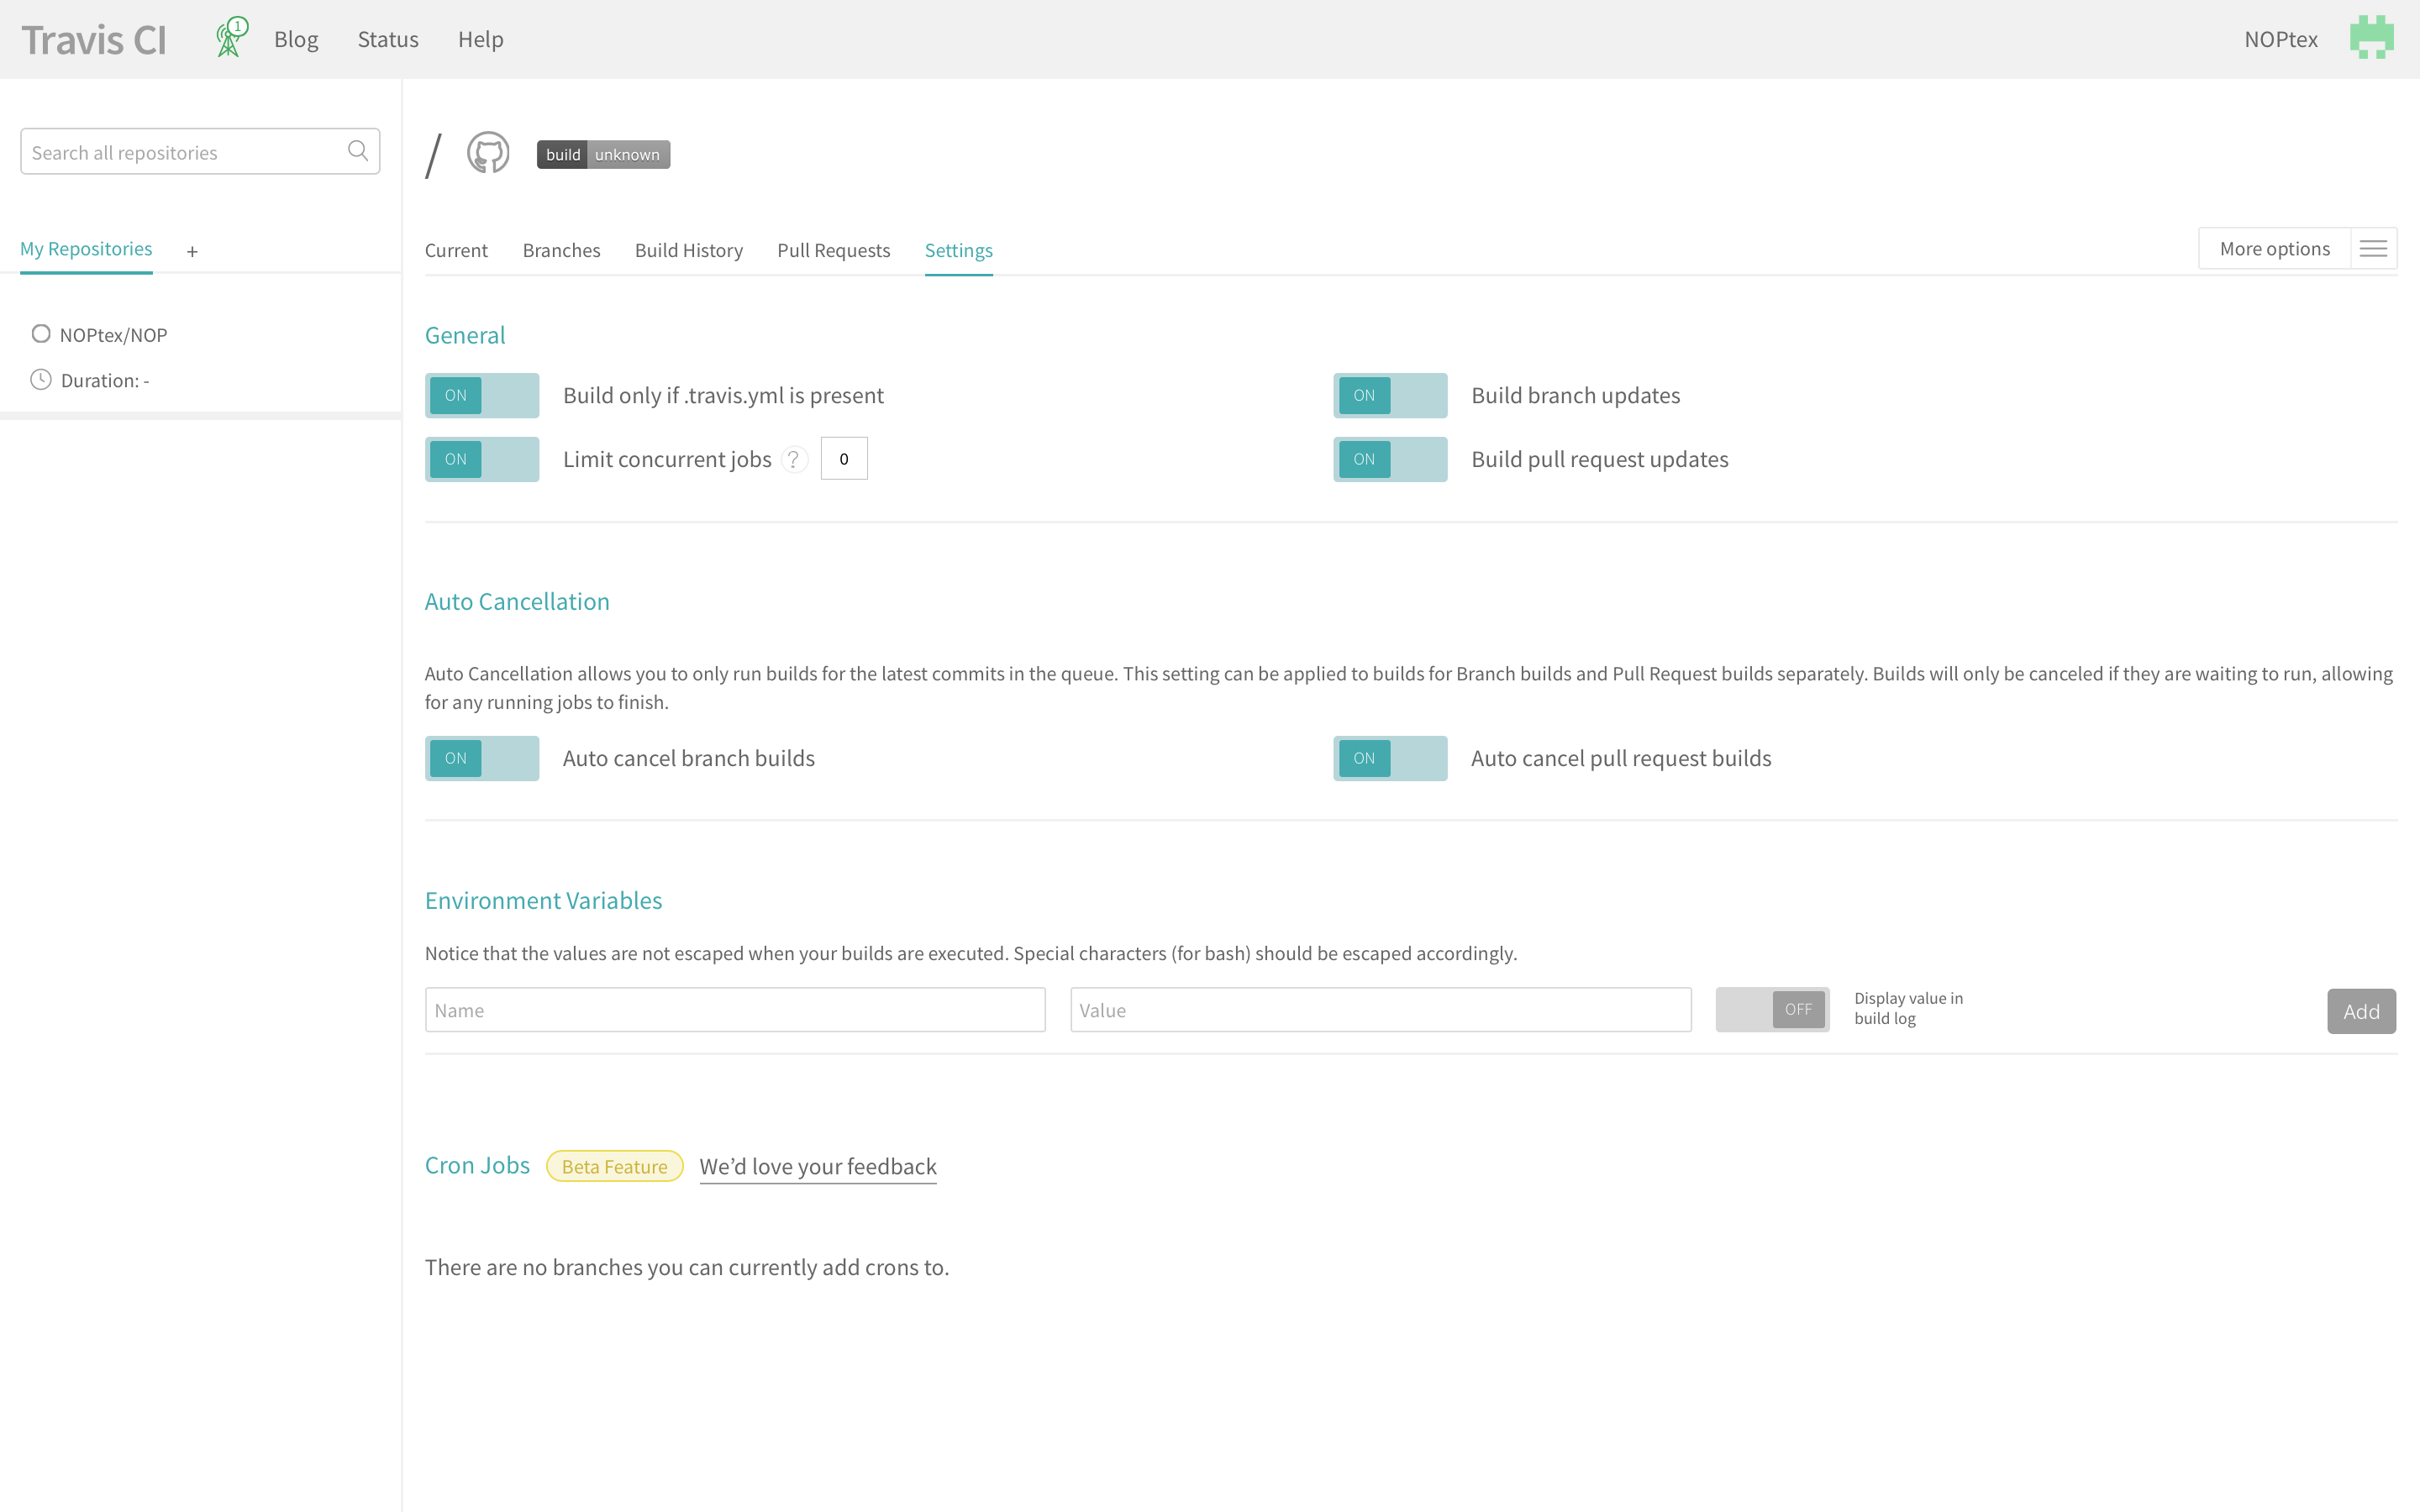
\includegraphics[width=1.0\textwidth]{./bilder/8TRAVISOptionsSET.png}
% \end{framed}
%
% \end{minipage}}
% \hfill
% \adjustbox{valign=t}{\begin{minipage}[t]{0.45\textwidth}
% \vspace{0pt}
% \huge
% Ich setze alle Häkchen weil:
% \begin{itemize}
%   \item nur releases Gebaut werden sollen \\ (Testen kann man lokal) \\ Alle anderen Build sollen abgebrochen werden.
%   \item Nur wenn .travis.yml vorhanden ist Build starten. \\(Einfaches deaktivieren über Git)
% \end{itemize}
% % \caption{Kapazität}
% \end{minipage}}
% \end{figure}
%
% \clearpage % GleitObjekte anzeigen
